\begin{figure}[t]
  \centering
  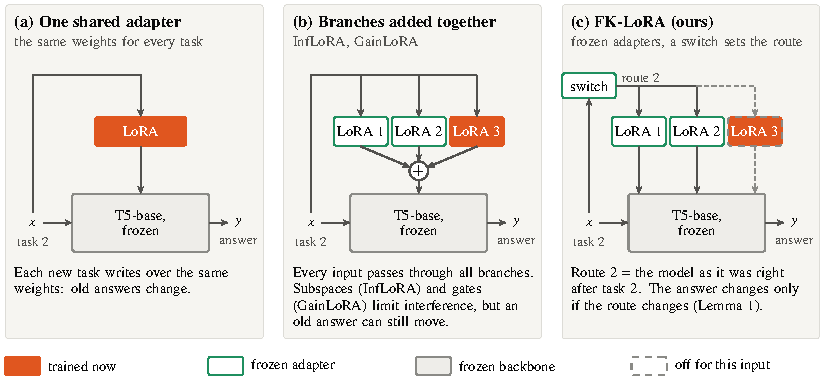
\includegraphics[width=\linewidth]{figures/overview}
  \caption{Three ways to add a task, shown while task~3 is being learned and an input of task~2 is
  answered. (a)~One shared adapter is trained again for each task, so old answers change.
  (b)~InfLoRA and GainLoRA add one branch per task, and every input passes through all branches
  (weighted by gates in GainLoRA); a chosen subspace or the gates limit what a new branch does to
  old inputs, but an old answer can still change. (c)~FK-LoRA never changes an adapter after its
  task has been learned, and a switch sets the route of each input: route~2 is the model as it was
  right after task~2, so the answer changes only if the route changes (Lemma~\ref{lem:route}).}
  \label{fig:overview}
\end{figure}
